\documentclass[a4paper]{article}

\usepackage{reportFormat}


\title{
	\Large {\sc Mech}4450 Aerospace Propulsion \\
	\Huge Major Assignment - Part 2
}

\author{
	Muirhead, Alex \\ \texttt{s4435062}
	\and
	Watt, Robert \\ \texttt{s4431151}
}

\date{\today}

\begin{document}

\pagenumbering{gobble}
\maketitle

% \tableofcontents

\vspace{10em}

\newpage
\pagenumbering{arabic}

\section{Methodology}
Combustion was modelled using the same model that was developed in part 1, however the temperature was calculated at each step along the solution from the heat released during combustion, rather than assuming a temperature profile ahead of time.

In order to calculate the temperature needed by the chemistry model, and also to calculate thrust, the total temperature and Mach number must be solved alongside the chemistry model. The additional equations to be solved are Eq.~\ref{eqn:dM2dx} and \ref{eqn:dTtdx}.
\begin{align}\label{eqn:dM2dx}
    \frac{\partial M^2}{\partial x} =M^2 \frac{1 + \frac{\gamma_b - 1}{2}M^2}{1-M^2}\left( -\frac{2}{A} \frac{\partial A}{\partial x} + \frac{1 + \gamma_b M^2}{T_t}\frac{\partial T_t}{\partial x} + \frac{4 \gamma_b M^2 C_f}{D}\right)
\end{align}
\begin{align}\label{eqn:dTtdx}
    \frac{\partial T_t}{\partial x} = - \frac{1}{c_{pb}}\sum_i \frac{\partial Y_i}{\partial x}h_{f,i}^\circ
\end{align}
Where
\begin{align}\label{eqn:spatial_mass_fraction_gradient}
    \frac{\partial Y_i}{\partial x} = \mathcal{M}_i \left\lbrace \frac{1}{\sum_j \left[X_j\right]\mathcal{M}_j} \frac{\partial \left[X_i\right]}{\partial x} - \frac{\left[ X_i \right]}{\left(\sum_j \left[X_j\right]\mathcal{M}_j \right)^2 }\sum_j \mathcal{M}_j\frac{\partial \left[ X_j \right]}{\partial x} \right\rbrace
\end{align}
and 
\begin{align}\label{eqn:spatial_concentratoin_gradient}
    \frac{\partial \left[X_j\right]}{\partial x} = \frac{1}{v(x)}\frac{\partial \left[X_j\right]}{\partial t}
\end{align}
Where \(\frac{\partial \left[X_j\right]}{\partial t}\) is calculated using the chemistry model, and \(v(x)\) is the velocity of the gas \(x\)~m along the combustion chamber. This converts the time derivatives computed by the chemistry model into spatial derivatives needed to model the combustion. The velocity can be found using the Mach number of the flow at \(x\).
\begin{align}\label{eqn:v(x)}
    v(x) = M(x) \sqrt{\gamma_b R_b T(x)}
\end{align}
Since \(T_t(x)\) and \(M(x)\) is solved for at each time step, \(T(x)\) can be calculated using isentropic flow relations (Eq.~\ref{eqn:T(x)}). This is needed by the chemistry model, and to calculate \(v(x)\).
\begin{equation}\label{eqn:T(x)}
    T(x) = T_t(x) \left[ 1 + \frac{\gamma_b  - 1}{2}M(x)^2 \right]^{-1}
\end{equation}
Thus, using all the above equations, a system of ordinary differential equations can be solved to give the mass fraction of each species, total temperature and Mach number at each point along the combustor.
\begin{align}
    \frac{\partial}{\partial x} 
    \begin{bmatrix}
    \left[ \ce{C_2 H_4} \right] \\
    \left[ \ce{O_2} \right] \\
    \left[ \ce{H_2 O} \right] \\
    \left[ \ce{CO} \right] \\
    \left[ \ce{CO_2} \right] \\
    \left[ \ce{N_2} \right] \\
    T_t\\
    M^2
    \end{bmatrix}
    =
    \begin{bmatrix}
        f_0 \left(T_t, M^2, \left[ X_i \right]\right)\\
        f_1 \left(T_t, M^2, \left[ X_i \right]\right)\\
        f_2 \left(T_t, M^2, \left[ X_i \right]\right)\\
        f_3 \left(T_t, M^2, \left[ X_i \right]\right)\\
        f_4 \left(T_t, M^2, \left[ X_i \right]\right)\\
        f_5 \left(T_t, M^2, \left[ X_i \right]\right)\\
        f_6 \left(T_t, M^2, \left[ X_i \right]\right)\\
        f_7 \left(T_t, M^2, \left[ X_i \right]\right)
    \end{bmatrix}
\end{align}
Additionally, the density of the flow at each point along the combustor can be calculated from conservation of mass.
\begin{align}
    \rho(x) = \frac{\dot{m}}{v(x) A(x)}
\end{align}
This density can then be used to calculate the pressure at each point in the combustor using the ideal gas law.
\begin{align}
    P(x) = \rho(x) R T(x)
\end{align}

\section{Results and Discussion}
\subsection{Inlet Modelling}
The flight conditions of the scramjet can be used to calculate properties of the gas entering the scramjet. Given values for the freestream flight conditions are listed in Table.~\ref{tab:freestream values}. 
\begin{table}[H]
    \centering
    \begin{tabu} spread 0cm {X[-1,l]X[-1,c]X[-1,r]}
        \toprule 
        \rowfont[c]{\bfseries} Property & Symbol & Value \\
        \midrule 
        Mach Number & \(M_0\) & 10 \\
        Static Temperature & \(T_0\) & \SI{220}{\K} \\
        Dynamic Pressure & \(q_0\) & \SI{50}{\kPa} \\
        Specific Gas Constant & \(R\) & \SI{287}{\J\per\kg\per\K} \\
        \bottomrule 
    \end{tabu}
    \caption{Freestream flight conditions}
    \label{tab:freestream values}
\end{table}
Using the static temperature to calculate the speed of sound \(a_0^2 = \gamma R T_0\), and the flight Mach number, the velocity of gas entering the scramjet is given as:
\begin{equation}
    v_0 = M_0 \sqrt{\gamma R T_0} = \SI{2973}{\m\per\s}
\end{equation}
% \begin{align}
%     v_0 &= M_0 \sqrt{\gamma R T_0}\\
%     &= 10 \times \sqrt{1.4 \times 287 \times 220}\\
%     &=\SI{2973}{\m\per\s}
% \end{align}
The vehicle operates at constant dynamic pressure, given by the relation \(q_0 = \frac{1}{2}\rho_0v_0^2\). With velocity known, this can be rearranged to give the inlet density, and subsequently pressure from the ideal gas law. 
\begin{gather}
    \rho_0 = \frac{2 q_0}{v_0^2} = \SI{0.011}{\kg\per\m\cubed} \\
    p_0 = \rho_0 R T = \SI{714.4}{\Pa}
\end{gather}
% \begin{align}
%     \rho_0 &= \frac{2 q_0}{v_0^2}\\
%     &= \frac{2 \times 50 \times 10^3}{2973^2}\\
%     &= \SI{0.011}{\kg\per\m\cubed}
% \end{align}
% And the ideal gas law can be used to calculate the pressure at the inlet.
% \begin{align}
%     P_0 &= \rho_0 R T\\
%     % &= 0.011 \times 287 \times 220\\
%     &= \SI{714.4}{\Pa}
% \end{align}
The specific heat at constant pressure for the air fuel mixture can be calculated from the ratio of specific heats and gas constant determined from the CFD modelling of the inlet.
\begin{align}
    c_{pb} &= \frac{\gamma_b}{\gamma_b - 1}Rb\\
    % &= \frac{1.3205}{1.3205 - 1}\times 288.45\\
    % &= \SI{1188.45}{\J\per\kg\per\K}\\
    &= \SI{1.18845}{\kJ\per\kg\per\K}
\end{align}
The density of the air fuel mixture at the inlet to the combustor can be calculated using the ideal gas law.
\begin{align}
    \rho_{3b} &= \frac{P_{3b}}{RT_{3b}}\\
    &= \frac{\num{70.09e3}}{288.45 \times 1400}\\
    &= \SI{0.174}{\kg\per\m\cubed}
\end{align}
The area of the inlet to the combustor, \(A_3\), can be calculated from conservation of mass applied to the fully mixed air-fuel mixture at the combustor inlet.
\begin{align}
    A_3 = \frac{\dot{m}}{\rho_{3b} v_{3b}}
\end{align}
CALCULATE THE REMAINING FLOW STATES


\subsection{Combustor Modelling}
The above system of equations was solved in python for three different inflow temperatures; 1000~K, 1237.63~K, and 1400~K. Plots of properties along the combustor are plotted in Figures

\begin{figure}[h]
    \centering
    \begin{subfigure}[h]{0.49\linewidth}
        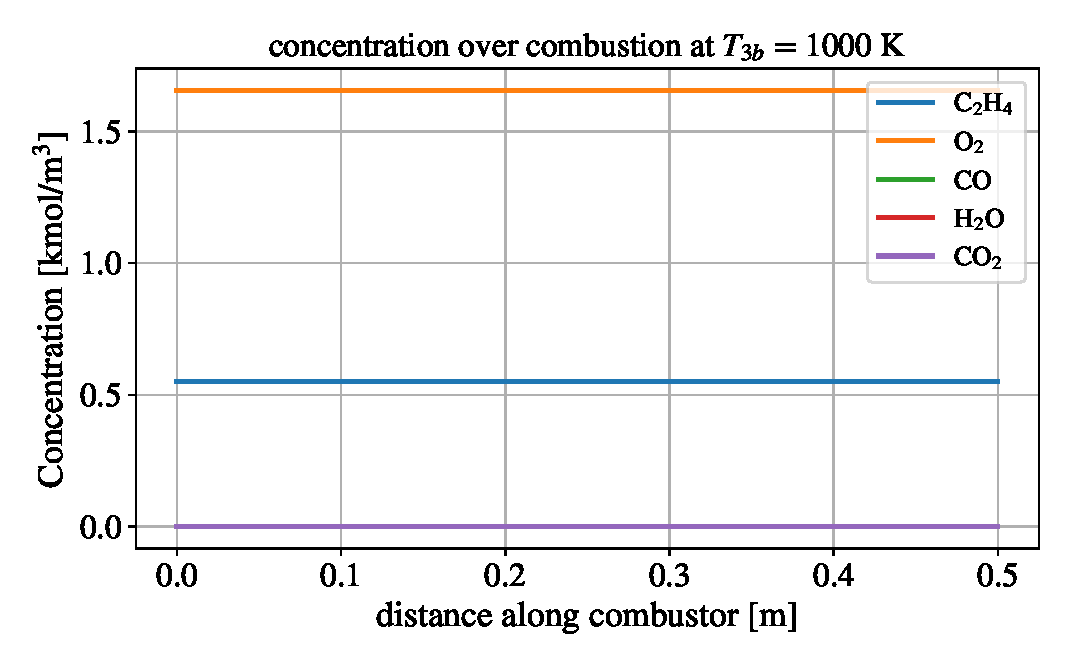
\includegraphics[width=\linewidth]{part_2_img/concentration_1000.pdf}
        \caption{Species Concentration}
        \label{subfig:concentration_1000}
    \end{subfigure}
    \begin{subfigure}[h]{0.49\linewidth}
        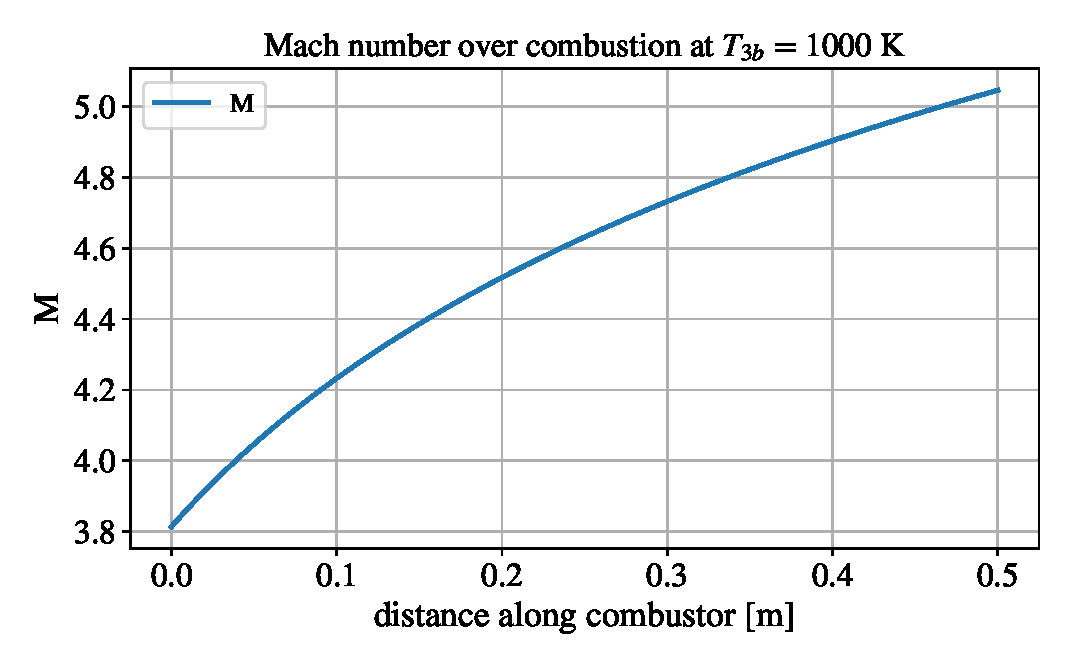
\includegraphics[width=\linewidth]{part_2_img/mach_1000.pdf}
        \caption{Mach number}
        \label{subfig:mach_1000}
    \end{subfigure}
    \begin{subfigure}[h]{0.49\linewidth}
        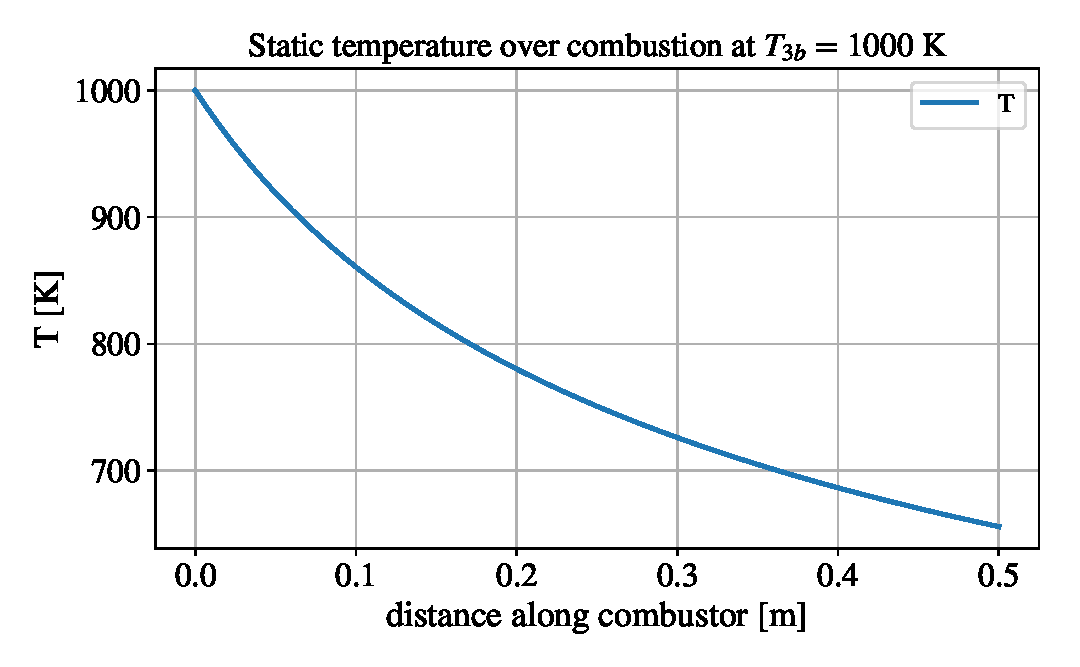
\includegraphics[width=\linewidth]{part_2_img/static_temp_1000.pdf}
        \caption{Static temperature}
        \label{subfig:temp_1000}
    \end{subfigure}
    \begin{subfigure}[h]{0.49\linewidth}
        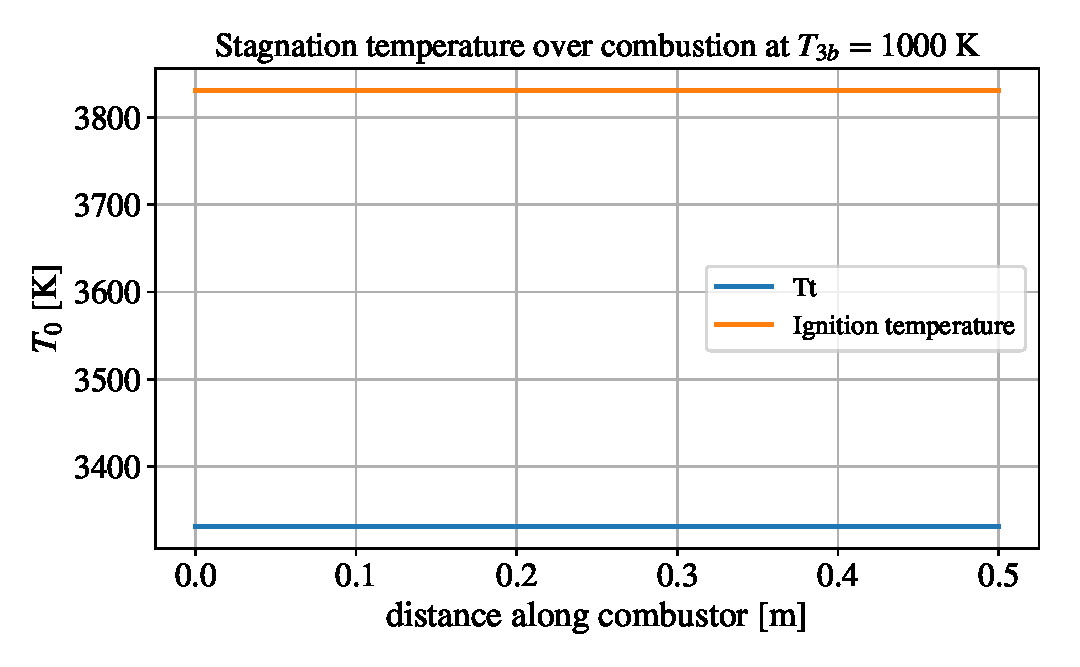
\includegraphics[width=\linewidth]{part_2_img/stag_temp_1000.pdf}
        \caption{Stagnation temperature}
        \label{subfig:stag_temp_1000}
    \end{subfigure}
     \begin{subfigure}[h]{0.49\linewidth}
        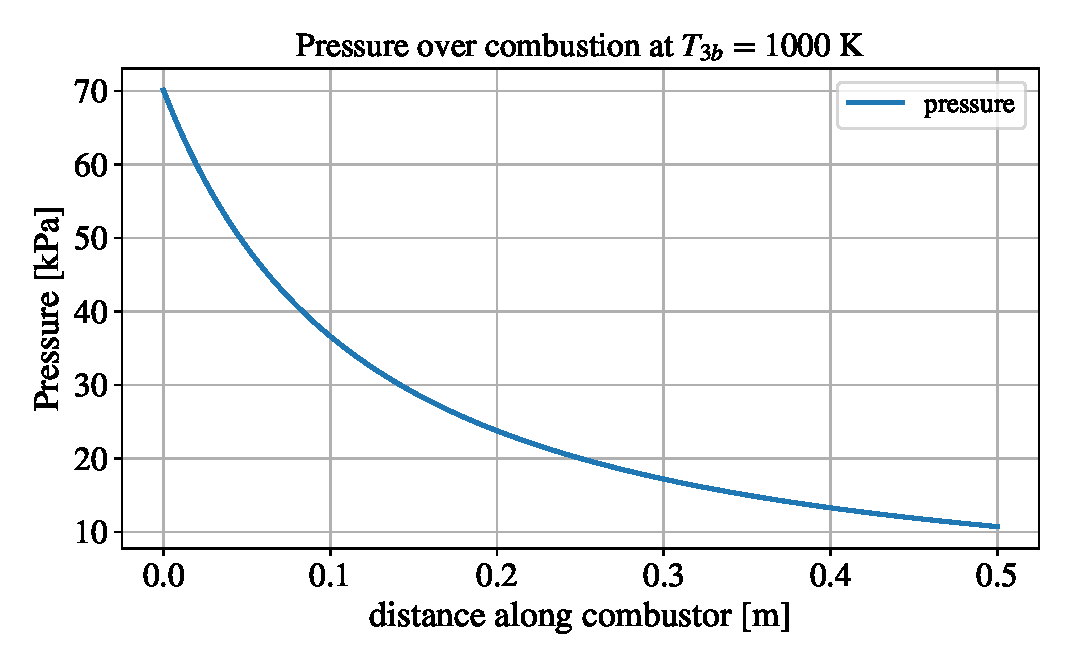
\includegraphics[width=\linewidth]{part_2_img/pressure_1000.pdf}
        \caption{Pressure}
        \label{subfig:pressure_1000}
    \end{subfigure}
    \caption{Properties over combustion at 1000~K}
    \label{fig:properties_1000}
\end{figure}

\begin{figure}[h]
    \centering
    \begin{subfigure}[h]{0.49\linewidth}
        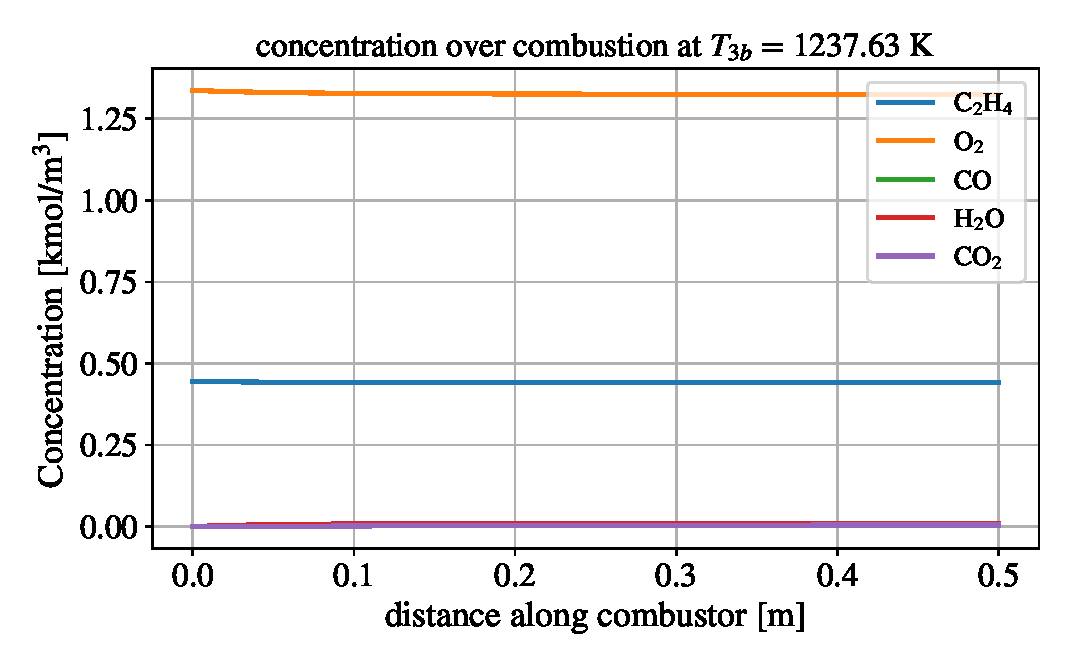
\includegraphics[width=\linewidth]{part_2_img/concentration_1237.63.pdf}
        \caption{Species Concentration}
        \label{subfig:concentration_1237}
    \end{subfigure}
    \begin{subfigure}[h]{0.49\linewidth}
        \includegraphics[width=\linewidth]{part_2_img/mach_1237.pdf}
        \caption{Mach number}
        \label{subfig:mach_1237}
    \end{subfigure}
    \begin{subfigure}[h]{0.49\linewidth}
        \includegraphics[width=\linewidth]{part_2_img/static_temp_1237.pdf}
        \caption{Static temperature}
        \label{subfig:temp_1237}
    \end{subfigure}
    \begin{subfigure}[h]{0.49\linewidth}
        \includegraphics[width=\linewidth]{part_2_img/stag_temp_1237.pdf}
        \caption{Stagnation temperature}
        \label{subfig:stag_temp_1237}
    \end{subfigure}
     \begin{subfigure}[h]{0.49\linewidth}
        \includegraphics[width=\linewidth]{part_2_img/pressure_1237.pdf}
        \caption{Pressure}
        \label{subfig:pressure_1237}
    \end{subfigure}
    \caption{Properties over combustion at 1237~K}
    \label{fig:properties_1237}
\end{figure}

\begin{figure}[h]
    \centering
    \begin{subfigure}[h]{0.49\linewidth}
        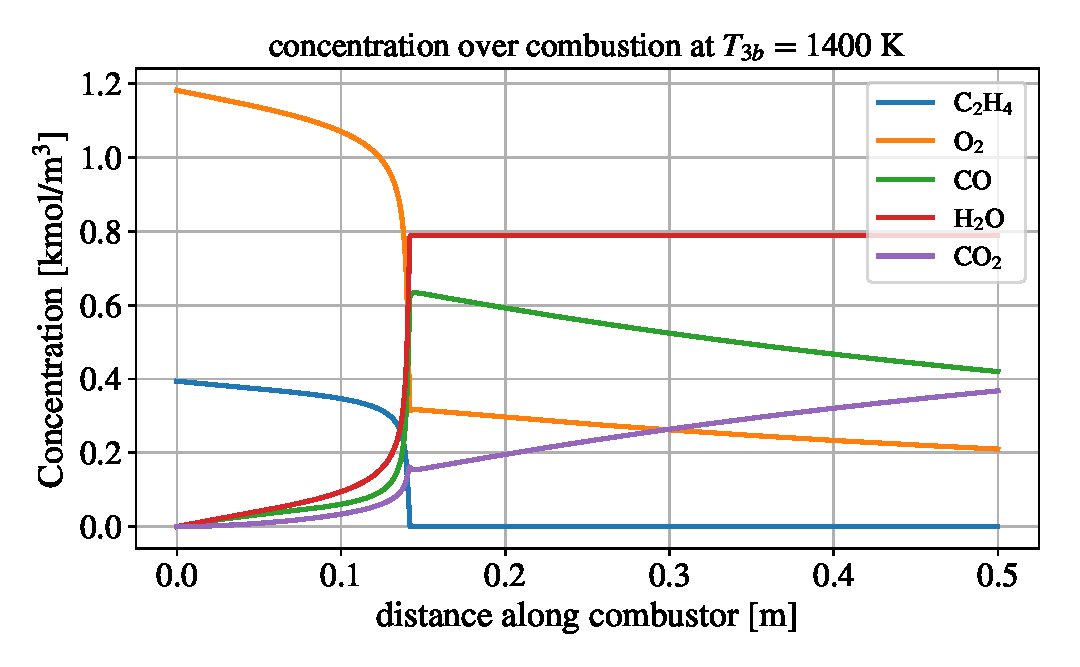
\includegraphics[width=\linewidth]{part_2_img/concentration_1400.pdf}
        \caption{Species Concentration}
        \label{subfig:concentration_1400}
    \end{subfigure}
    \begin{subfigure}[h]{0.49\linewidth}
        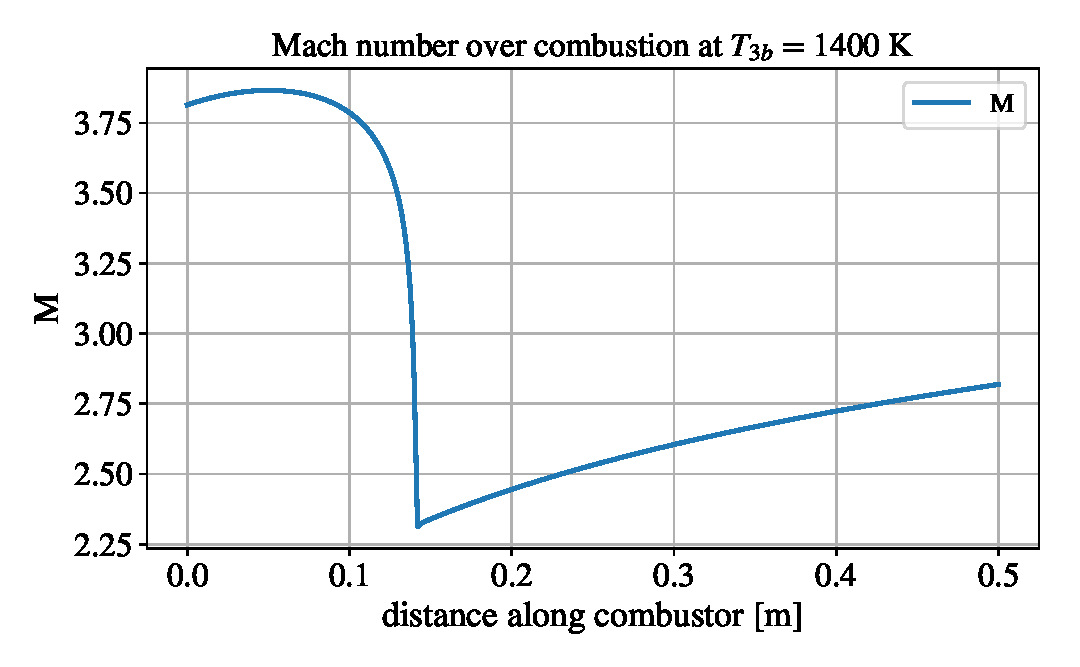
\includegraphics[width=\linewidth]{part_2_img/mach_1400.pdf}
        \caption{Mach number}
        \label{subfig:mach_1400}
    \end{subfigure}
    \begin{subfigure}[h]{0.49\linewidth}
        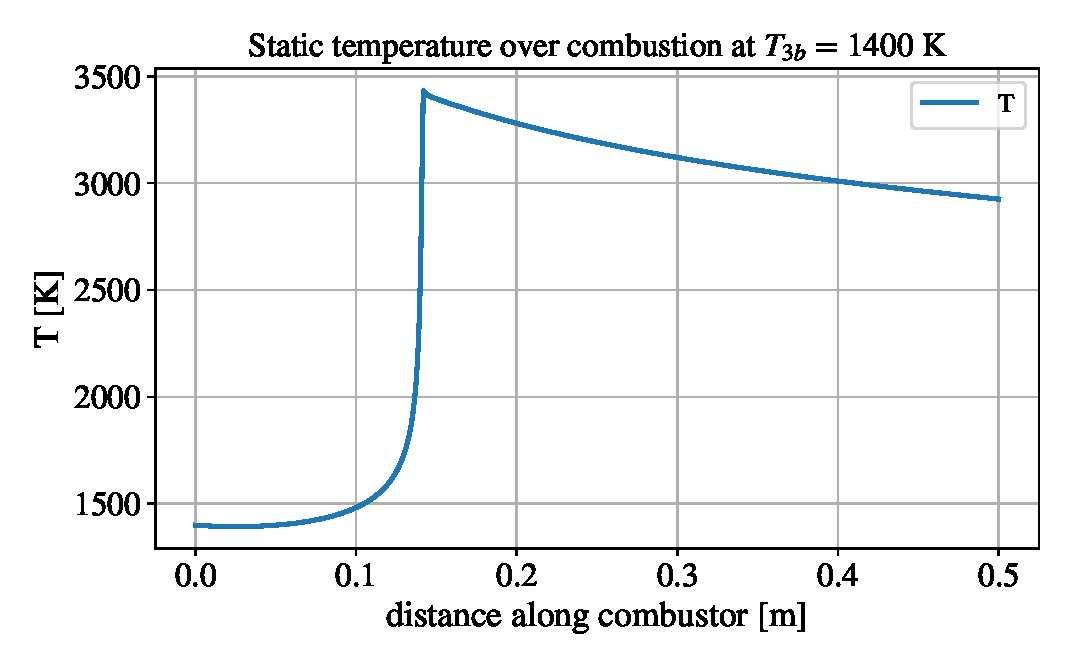
\includegraphics[width=\linewidth]{part_2_img/static_temp_1400.pdf}
        \caption{Static temperature}
        \label{subfig:temp_1400}
    \end{subfigure}
    \begin{subfigure}[h]{0.49\linewidth}
        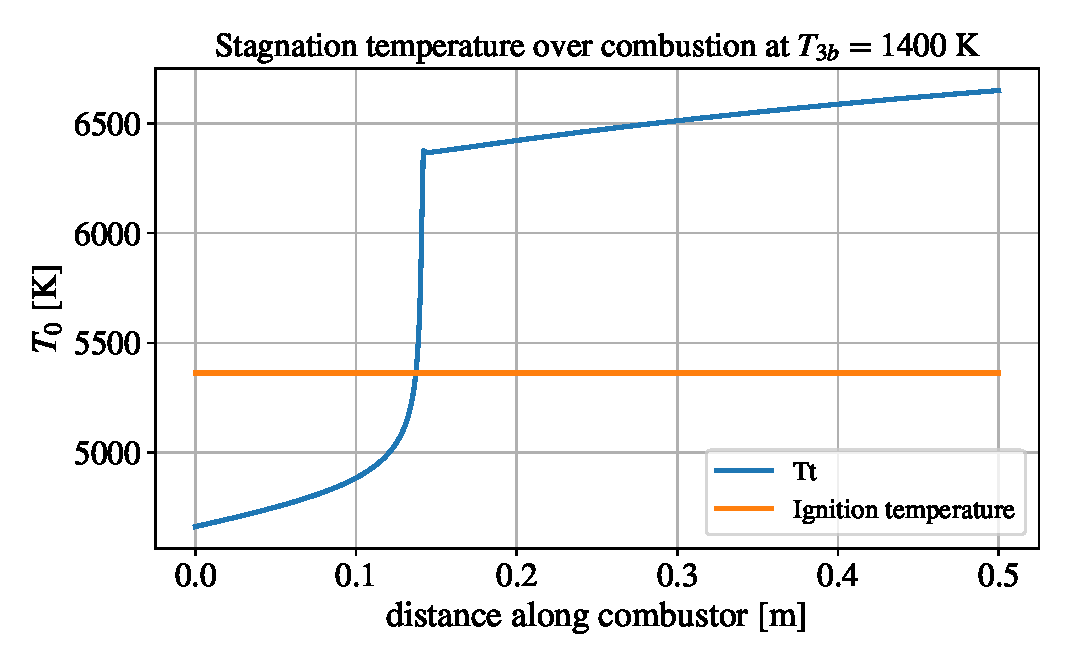
\includegraphics[width=\linewidth]{part_2_img/stag_temp_1400.pdf}
        \caption{Stagnation temperature}
        \label{subfig:stag_temp_1400}
    \end{subfigure}
     \begin{subfigure}[h]{0.49\linewidth}
        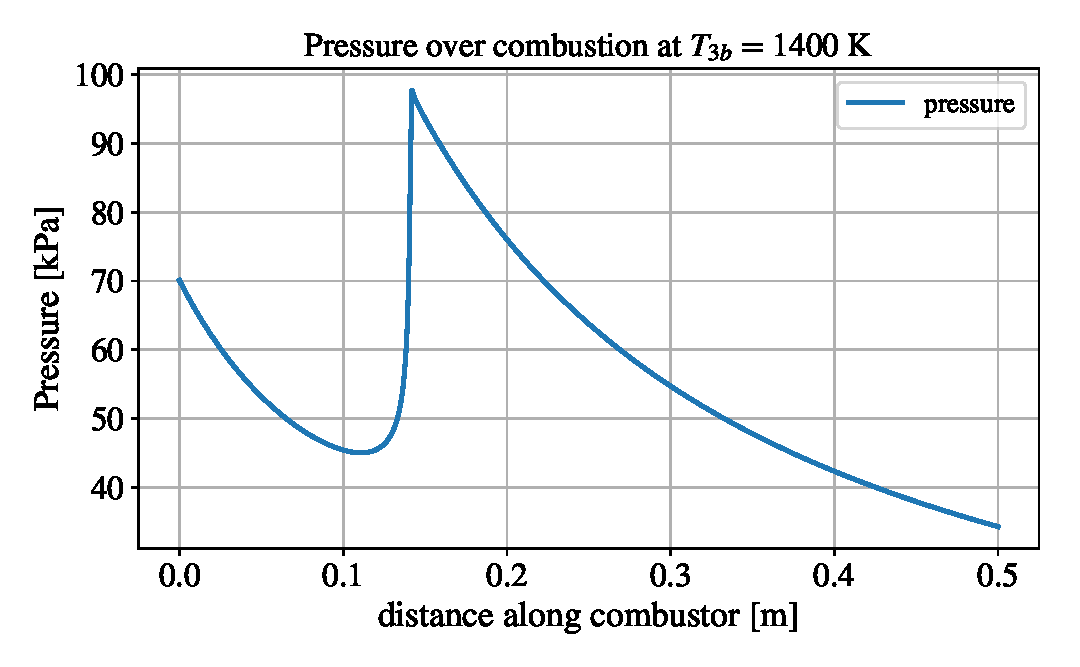
\includegraphics[width=\linewidth]{part_2_img/pressure_1400.pdf}
        \caption{Pressure}
        \label{subfig:pressure_1400}
    \end{subfigure}
    \caption{Properties over combustion at 1400~K}
    \label{fig:properties_1400}
\end{figure}

\subsection{Nozzle Modelling}

\subsection{Overall Performance and Discussion}

\end{document}